\subsection*{Ejemplo 1: un simple problema de regresión}

El siguiente código en MATLAB representa un conjunto de datos sobre el cancer y la cantidad de cigarrillos que se fuma por día. Se realiza una regresión lineal para predecir la mejor forma que se adapte a los datos (minimize los errores) y además una regresión de grado 15. En la figura \ref{fig:1} se grafica los resultados

\begin{lstlisting}
clc
clear all
close all

%% Ejemplo 1
cig = 0:1:32;
cancer = 1.7*cig + 22 + 5*randn(size(cig));

fig = figure;
theme(fig, 'light')
%Casos de cancer
plot(cig, cancer, 'b')
hold on;

%Hacemos una regresion lineal
lin = polyfit(cig, cancer, 1);
cancer_est = polyval(lin, cig);
plot(cig, cancer_est, 'r')
xlabel('Cigarrillos por dia')
ylabel('Casos de cancer')

%Hacemos una regresion de grado 15
orden15 = polyfit(cig, cancer, 15);
cancer_est15 = polyval(orden15, cig);
plot(cig, cancer_est15, 'g')
\end{lstlisting}

\begin{figure}[ht!]
    \centering
    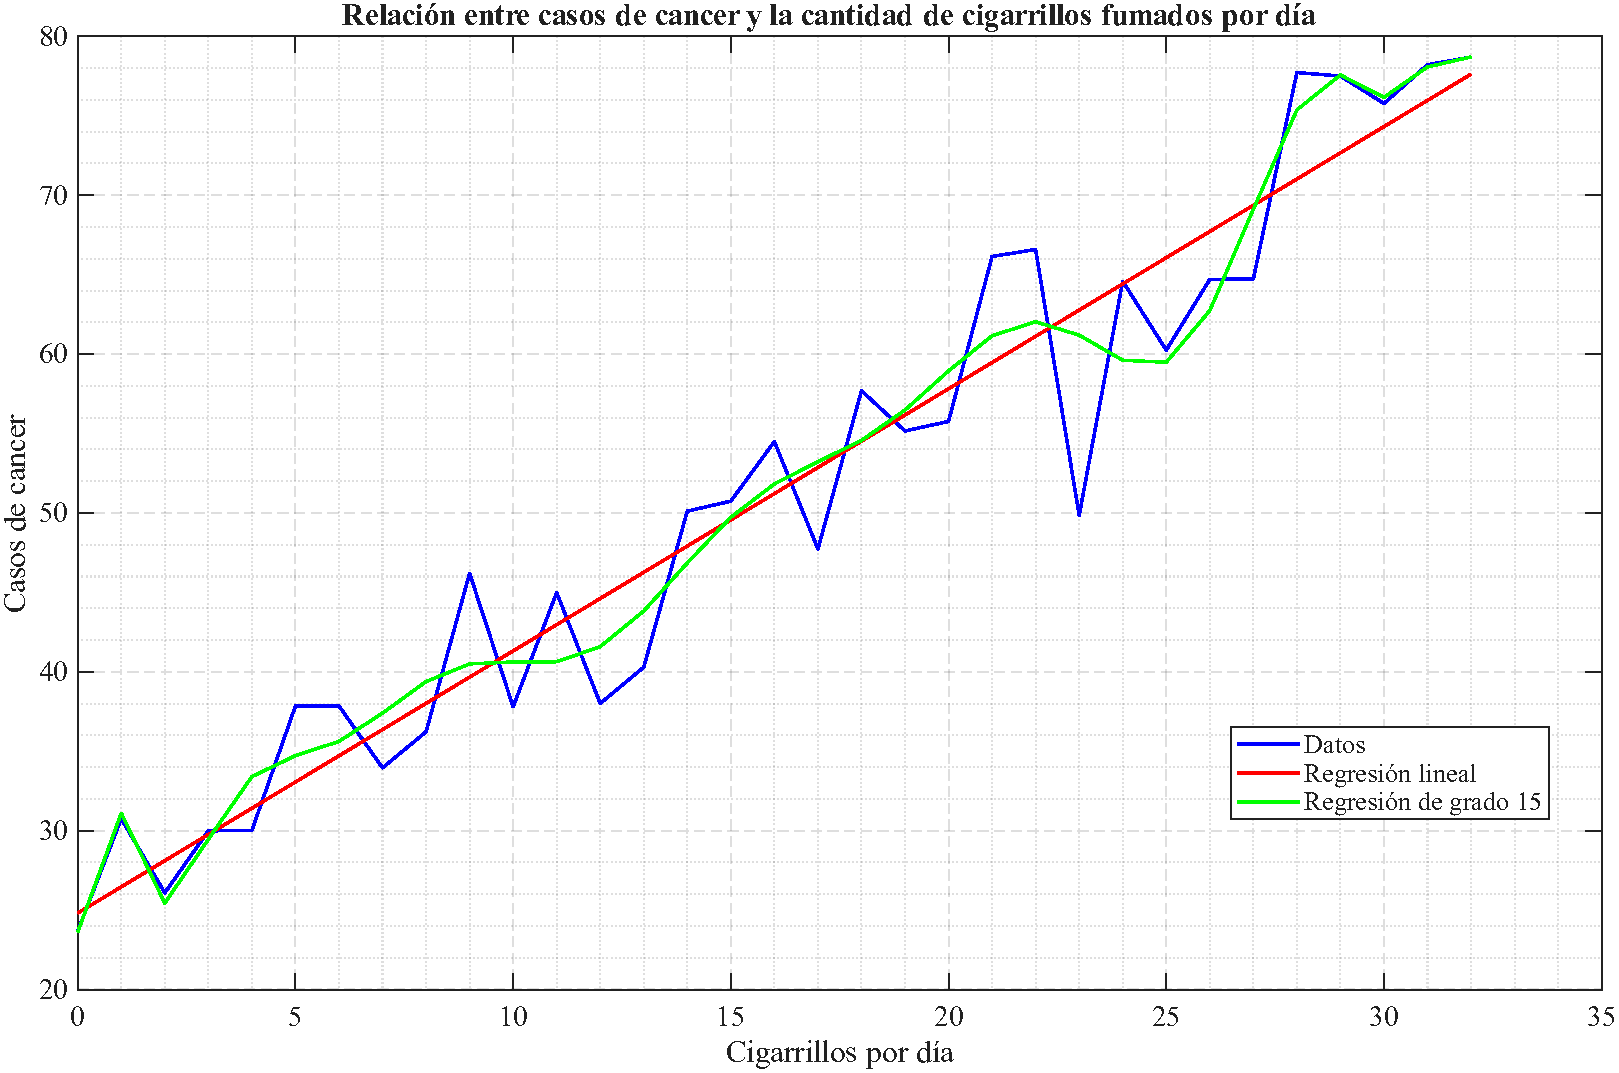
\includegraphics[width=0.8\textwidth]{imagenes/cancerplot.pdf}
    \caption{Gráfico de los datos}
    \label{fig:1}
\end{figure}

El modelo lineal tiene la ventaja computacional y que visualmente representa una función simple, marcando la tendencia general de los datos. En cambio, el polinomio de mayor grado representa la ventaja de que se ajustará más a los datos. Aunque parezca más razonable usar un polinomio de mayor grado, este representa una clara desventaja. Según \textit{Steven C. Chapra & Raymond P. Canale : Método Numéricos para Ingenieros} (Capítulo 17, sección 17.2.1):

\begin{displayquote}
Un problema potencial en la implementación de la regresión polinomial en la computadora es que las ecuaciones normales algunas veces están mal condicionadas. Esto se presenta especialmente cuando se planten polinomios de grado superior. En tales casos, los coeficientes calculados pueden ser altamente susceptibles al error de redondeo y, en consecuencia, los resultados serían inexactos.
\end{displayquote}

Donde las ecuaciones normales son un conjunto de ecuaciones (que depende del grado del polinomio) lineales simultáneas. Por último, se observa que la variable \texttt{cancer} tiene un término random y en la regresión polinómica esto puede representar un problema causando el sobreajuste (\textit{Overfitting}): condición donde en un modelo empieza a describir el ruido en lugar de la relación entre las variables. Este problema se puede ver en la gráfica de arriba. 

\subsection*{Predicción de series temporales}

La siguiente figura representa el precio de la soja y los modelos empleados para predecir el precio durante los próximos 3 años.

\begin{figure}[ht!]
    \centering
    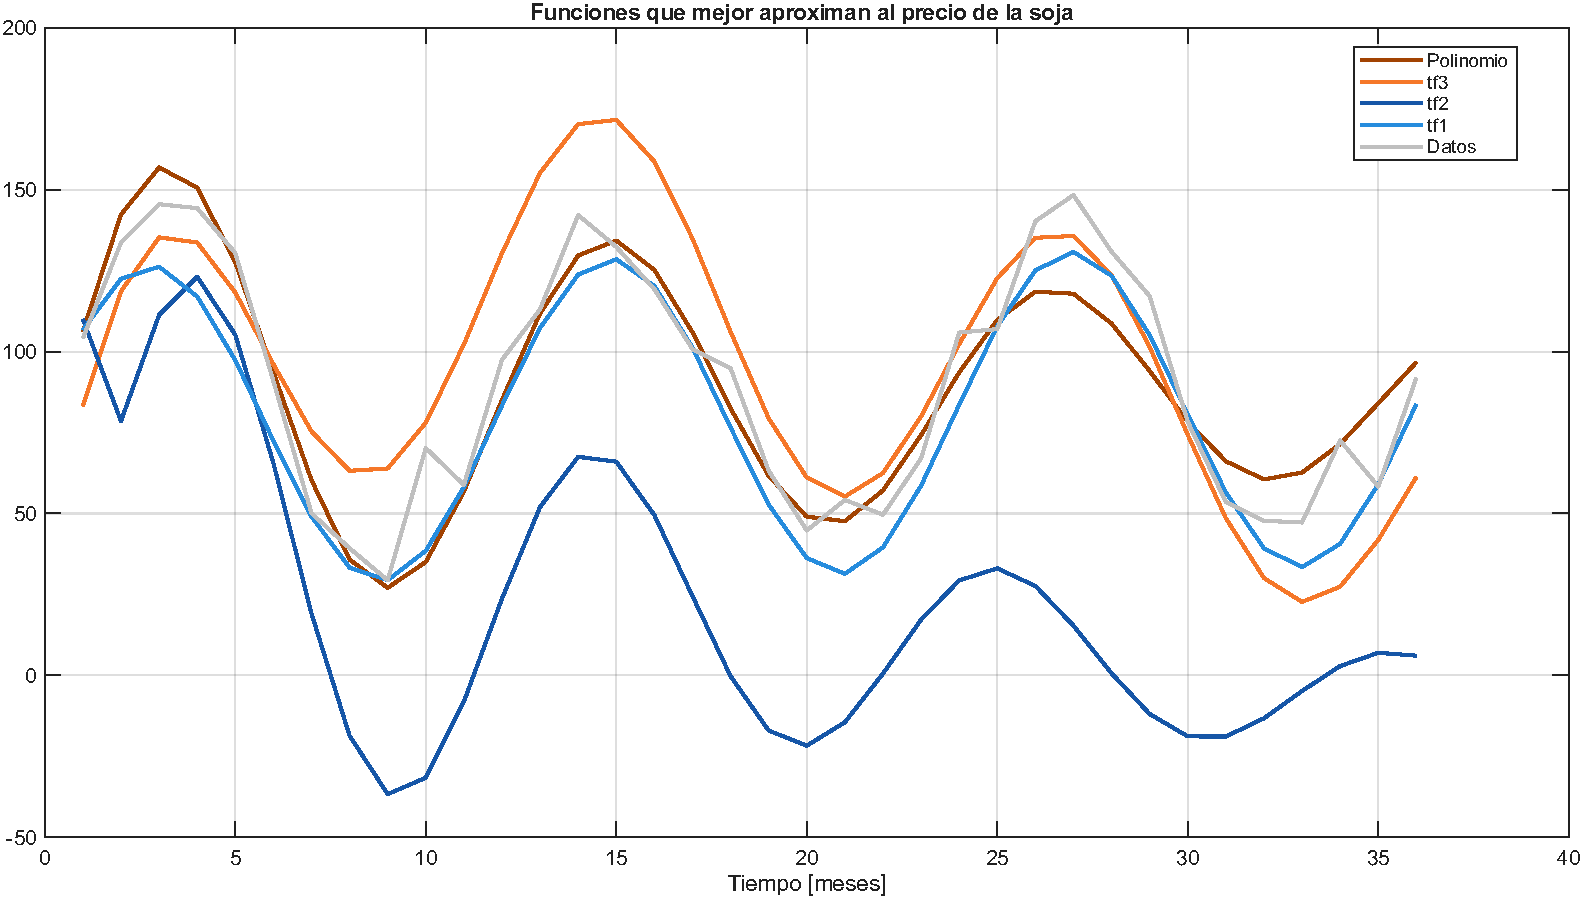
\includegraphics[width=0.9\textwidth]{imagenes/ploteosoja.pdf}
    \caption{Modelos que mejor estiman el precio de la soja durante los próximos años}
    \label{fig:2}
\end{figure}


De los modelos empleados, el que mejor estima es el polinomio con un \textit{Best Fit} de 63.59. Para tf1 58.21, tf2 -107.4 y tf3 35.67. Los modelos pueden superar el valor de 80 pero esto implica jugar con los distintos modelos hasta que encaje dentro de los valores de 80 (anteriormente realicé una prueba y obtuve un Best Fit de 82, pero al tener un término randn en la variable \texttt{y} éste varía con cada compilación que realice). 

Para tf1, la función transferencia obtenida fue:

\begin{equation}
    \frac{21.3s + 0.04801}{s^2 + 1.167\times10^{-9}s + 0.2707}
\end{equation}

\noindent con 2 polos y un cero. Para tf2 

\begin{equation}
    \frac{14.3s^2 + 32.51 s - 1.091}{s^3 + 2.413s^2 + 0.6228 s + 0.823}
\end{equation}

\noindent con 3 polos y 2 ceros. Para tf3

\begin{equation}
    \frac{15.1 s^3 + 49.35 s^2 + 7.818 s - 0.1673}{s^3 + 0.2033s^2 + 0.2728s + 0.05042}
\end{equation}

\noindent con 3 polos y 3 ceros. Por último, el polinomio tiene la estructura $A(z)y(t) = B(z)u(t) + e(t)$, donde

\begin{align}
    &A(z) = 1 - 0.6494\frac{1}{z} - 0.4911 \frac{1}{z^2} + 0.5377 \frac{1}{z^3} + 0.2277\frac{1}{z^4}\\
    &B(z) = 17.81 \frac{1}{z} - 17.78\frac{1}{z^4}
\end{align}


Se observa que a medida que el sistema es más complejo (de mayor orden) pueden resultar peores que los sistemas menos complejos, tal como sucede con tf1 y tf3.


\subsection*{Encontrar padrones con redes neuronales}

Veamos la siguiente figura

\begin{figure}[ht!]
    \centering
    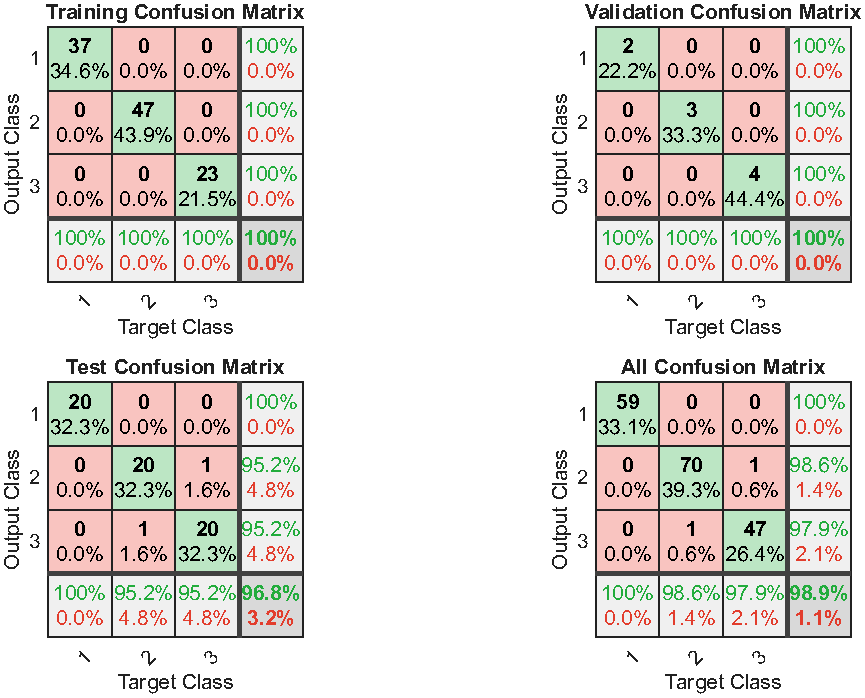
\includegraphics[width=0.8\textwidth]{imagenes/red_neuronal.pdf}
    \caption{Plot confusion}
    \label{fig:3}
\end{figure}


\noindent \textbf{Training Confusion Matrix}
\vspace{0.2cm}

Corresponde a los datos utilizados para ajustar los pesos y sesgos de la red, es decir, para que aprenda a clasificar. En la imagen figura que hubo 37 aciertos para la clase 1, 47 para la clase 2 y 23 de la clase 3, lo que equivale al 100\% de clasificación en las muestras.


\vspace{0.4cm}
\noindent \textbf{Validation Confusion Matrix}
\vspace{0.2cm}

El conjunto de validación se utiliza para supervisar el aprendizaje y ayudar a decidir cuándo detenerlo, evitando seguir ajustado la red cuando empeora su comportamiento fuera del conjunto de entrenamiento. Dicha matriz depende de la cantidad de datos y cómo estos influyen sobre el porcentaje de aciertos.


\vspace{0.4cm}
\noindent \textbf{Test Confusion Matrix}
\vspace{0.2cm}

Evalúa el comportamiento de la red con datos que no se utilizaron para ajustar sus parámetros ni para decidir cuándo detener el entrenamiento. Es decir, la red reconoció 62, donde 2 de ellos (números fuera de la diagonal principal) son errores. 

\vspace{0.4cm}
\noindent \textbf{All Confusion Matrix}
\vspace{0.2cm}


Reúne los resultados de entrenamiento, validación y prueba. El 98.9\% incluye las muestras de entrenamiento.

Por último, aumentar o disminuir la cantidad de neuronas ocultas no garantiza mejores predicciones (sobreajuste).